\section{Test Generation}
\label{sec:approach}

Given an operation ${\cal O}$ and a target rule part $r$ in ${\cal O}$, our
technique attempts to generate a \textit{test sequence}, consisting of an
operation sequence and test data, that \textit{covers} $r$---that is, the
sequence produces all input entities of ${\cal O}$ in appropriate object states
to ensure that the precondition of $r$ is satisfied. The challenge is to search
for a covering sequence efficiently from a large set of candidate sequences. For
example, one of our experimental subjects, \subject{Cebu-pacific}, has eight
operations that accept an entity \subject{Ticket} as input and modify
it. Therefore, any sequence composed using one or more of these operations can
be a candidate sequence; however, different sequences and orderings produce
different object states of \subject{Ticket}. Our technique addresses this
challenge by exploring the large search space efficiently, in a goal-directed
manner, by ignoring sequences that are not likely to cover the target rule.

%% In general, it is often challenging to identify a test sequence that covers $r$,
%% since there can be a large number of candidate sequences and only a few
%% sequences produce desired object states that help cover $r$. For example, in one
%% of our subjects \subject{Cebu-pacific}, there are eight operations that accept
%% an entity \subject{Ticket} as input and modify that entity. Therefore, any
%% sequence composed using one or more of these operations is a valid sequence,
%% however, different sequences and also different orderings of those sequences
%% produce different object states of the \subject{Ticket} entity.  Our technique
%% addresses this challenge by efficiently exploring the large search space via
%% composing sequences incrementally.

%% Overall, our technique first enumerates sequences of operations (along with
%% selected rule parts in those operations) that create all input entities of
%% ${\cal O}$.  Next, for each sequence, it checks whether the sequence generates
%% the desired object states (for all input entities of ${\cal O}$) so that $r$ is
%% covered. If the sequence is satisfiable, our technique infers test data for all
%% inputs that are of primitive and enumerated types.  Otherwise, it identifies an
%% entity $e$ and its attribute $attr$ that needs to be modified to achieve the
%% desired object state. Next, it identifies candidate operations that modify
%% $attr$, composes new sequences using those candidate operations, and further
%% checks whether those new sequences are satisfiable. Our technique repeats this
%% process until it identifies a satisfiable sequence or reaches a user-defined
%% threshold of the maximum number of sequences to be explored.

\subsection{Terminology}

Before presenting the test-generation algorithm, we introduce some terminology
and definitions: we discuss two types of graphs (the dependence graph and the
operation flow graph) and define abstract and concrete operation sequences.

\subsubsection{Graphs}

%\vskip -10pt
\paragraph*{Dependence Graph} A \textit{dependence graph} is a directed graph
that captures interactions of operations with entities: nodes in the graph
represent operations and entities, whereas edges represent creates, reads, and
modifies relations.  
%A \textit{creates edge} or a \textit{modifies edge} from an
%operation to an entity indicates that the operation creates or modifies that
%entity; a \textit{reads edge} from an entity to an operation indicates that the
%operation reads the entity.  
Figure~\ref{fig:sample-app} shows the dependence graph for our example application.

%% While composing sequences, our technique uses this graph to ensure that the
%% dependencies among operations are satisfied.  Figure~\ref{fig:sample-app}
%% shows the dependency graph for our example application.

\begin{figure}[t]
\centering
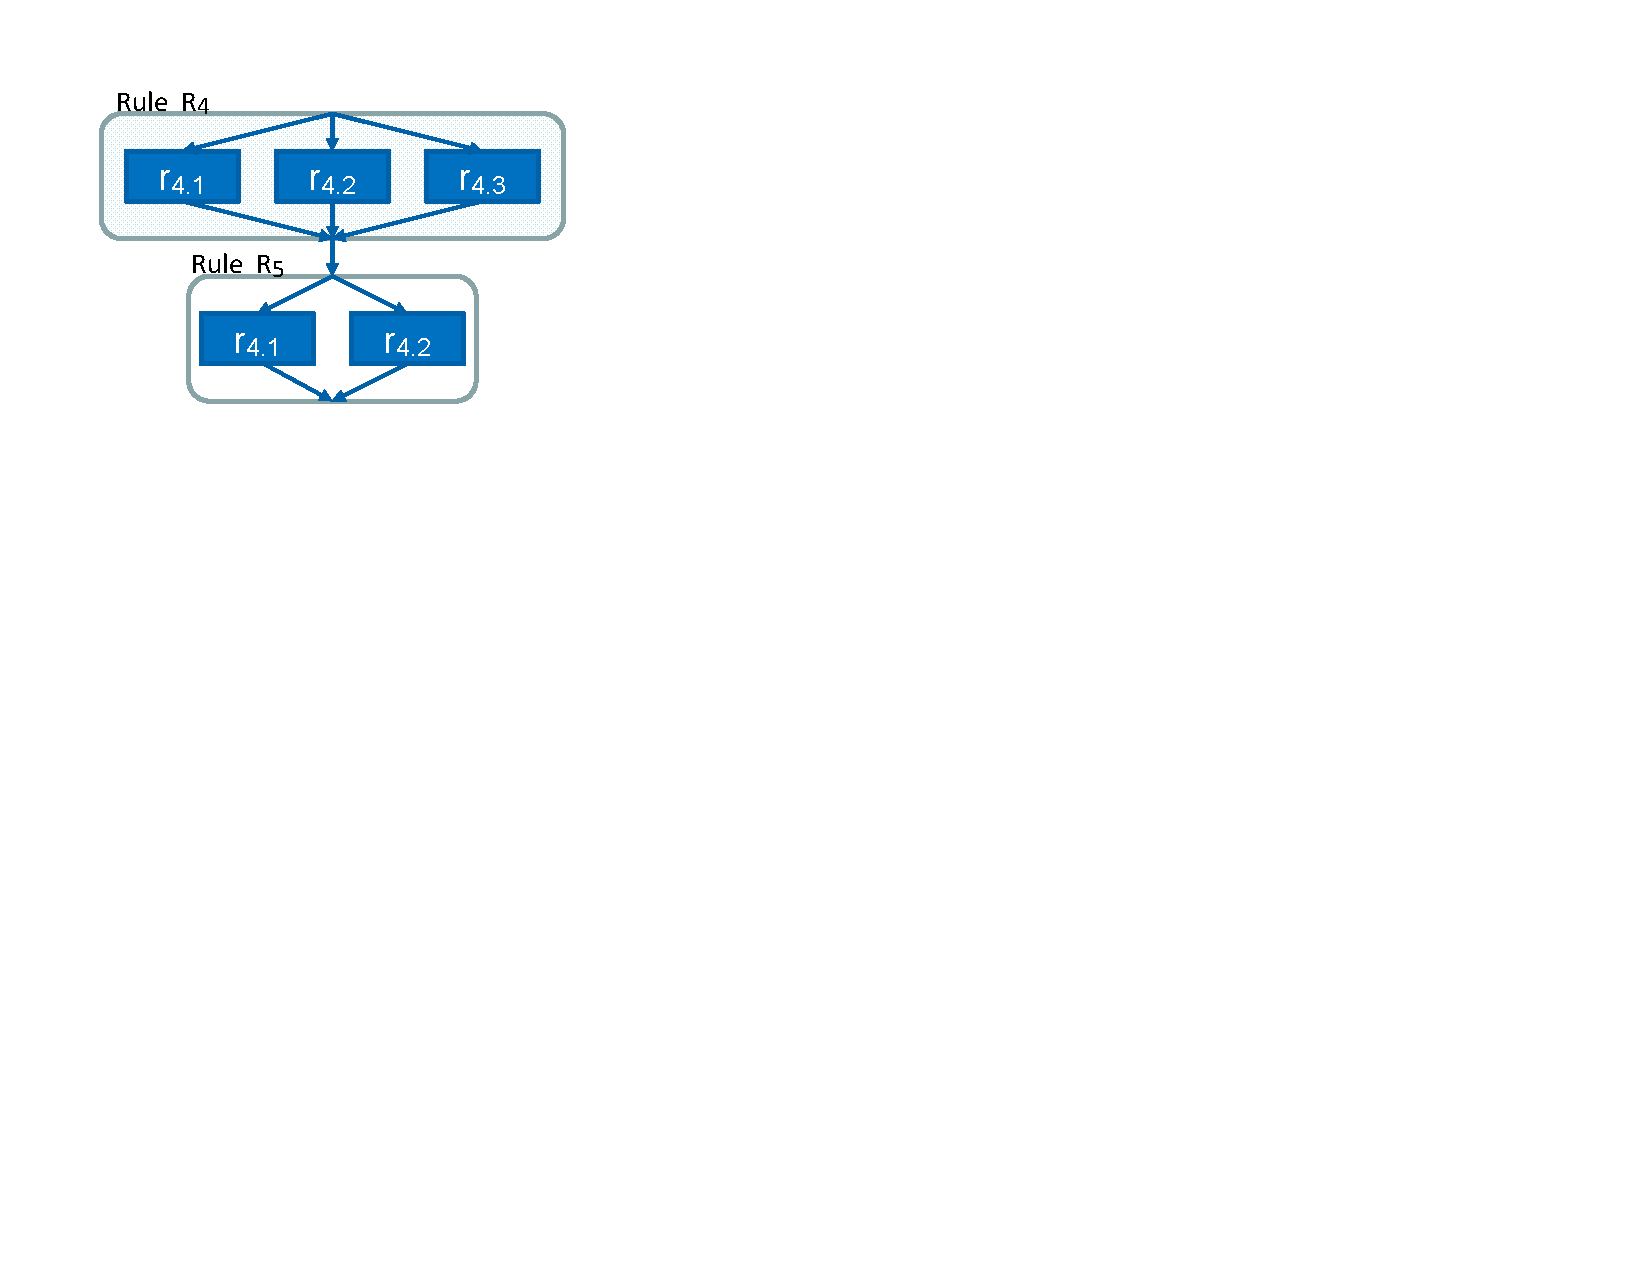
\includegraphics[trim=47 390 520 47,clip,width=.45\columnwidth]{figs/cfg-example.pdf}
\vspace*{-20pt}
\caption{Operation flow graph for \subject{GenerateInvoice}.}
\label{fig:cfg}
\end{figure}

%\vskip -7pt
\paragraph*{Operation Flow Graph} To identify combinations of rule parts (within
an operation) that create different object states of entities, we model an
operation as a flow graph. The \textit{operation flow graph} is a directed graph
consisting of rule subgraphs---one per rule of the operation---and edges
representing flow among the subgraphs. A \textit{rule subgraph} consists of a
unique entry point, a unique exit point, and nodes that represent rule parts;
the subgraph contains an edge from the entry point to each node and an edge from
each node to the exit point.  Figure~\ref{fig:cfg} illustrates the operation
flow graph for \subject{GenerateInvoice} with two rules, $R_4$ and $R_5$, which
have three and two rule parts, respectively.

Because preconditions of all rule parts in a rule are disjoint (Property~1,
Section~\ref{sec:model}), control flow through a rule covers exactly one rule
part.  The rule subgraph captures this aspect by representing each rule as a
choice among its rule parts. Moreover, because there are no data dependences
between rules of an operation (Property~3, Section~\ref{sec:model}), the rule
subgraphs can be composed in any order in the operation flow graph (\ie all
orderings are equivalent).

\subsubsection{Operation Sequences}

%\vskip -10pt
\paragraph*{Abstract Sequence} An \textit{abstract sequence} is a sequence of
operations describing flow of objects among the operations such that all
variables that represent instances of entities are defined and the remaining
variables (of enumerated and primitive types) need not be defined. An example
abstract sequence for \subject{GenerateInvoice} is:

\vspace*{-4pt}
{\scriptsize
\begin{alltt} 
 State st; BalanceType bt; int price;
 Customer cust = CreateCustomer(st, bt);
 Order ord = CreateOrder(cust);	 
 Item item = CreateItem(price);
 Order ord1 = AddItemToOrder(ord, item);
 Invoice inv = GenerateInvoice(ord1);  
\end{alltt}
}
\vspace*{-4pt}

All entity instances are initialized within the sequence.  If an operation
creates or modifies multiple entities, we represent those entities as arguments
prefixed with the keyword \subject{out}.

\vskip -7pt
\paragraph*{Concrete Sequence} A \textit{concrete sequence} constrains an
abstract sequence with selected rule parts for each operation. For an operation,
multiple rule parts can be selected from different rules of the operation. Our
technique uses concrete sequences to generate test data by leveraging 
constraint solving: it builds a logical formula from concrete sequences using
preconditions and postconditions of all rule parts, and uses a solver to check
whether the formula is satisfiable. An example concrete sequence for the
preceding abstract sequence is:

\vspace*{-4pt}
{\scriptsize
\begin{alltt} 
 State st; BalanceType bt; int price;
 Customer cust = CreateCustomer(st, bt) [\(r\sb{1.1}\)];
 Order ord = CreateOrder(cust) [\(r\sb{3.1}\)];	
 Item item = CreateItem(price) [\(r\sb{2.1}\)];
 Order ord1 = AddItemToOrder(ord, item) [\(r\sb{7.1}\)];
 Invoice inv = GenerateInvoice(ord1) [\(r\sb{4.1}\)];  
\end{alltt}
}
\vspace*{-5pt}

\subsection{The Algorithm}
\label{sec:technique}

The test-generation algorithm (shown as Algorithm~\ref{alg:guidedsearch}) takes
as inputs an operation ${\cal O}$ and a rule part $r$, and generates a concrete
sequence $seq$ that cover $r$. To illustrate the algorithm, we consider rule
part $r_{4.2}$ of \subject{GenerateInvoice}. For brevity, we omit details such
as exiting the main loop (lines~6--13) when the user-defined threshold of
maximum number of sequences to be explored is reached. We first explain the core
algorithm and then present the optimization that uses unsatisfied cores to
exploring the search space efficiently.

\begin{algorithm}[t]
\footnotesize
\SetAlgoVlined
\KwIn{Operation ${\cal O}$, Rule part $r$}
\KwOut{Concrete sequence $seq$ or $null$}
\BlankLine

\nl Let $q$ represents a queue of concrete sequences\;
\nl Generate all initialization sequences $iseqs$ for ${\cal O}$\;
\nl \ForEach {sequence $iseq \in iseqs$}
{
		\nl Generate all concrete sequences $cseqs$ for $iseq$\;
		\nl Add $cseqs$ to queue $q$\;
} 

\nl \While { q not empty }
{
		\nl Dequeue sequence $cseq$ from $q$\;
		\nl Check whether $cseq$ is satisfiable\;
		\nl \If {satisfiable}
		{
				\Return $cseq$\;
		}
		
		\nl Identify candidate operations $ops$\;		
		\nl \ForEach {operation $op \in ops$}
		{
			\nl Generate new sequences $nseqs$ by adding $op$ to $cseq$\;
			\nl Add all $nseqs$ to queue $q$\;
		}
}

\Return $null$\;
		
\caption{\label{alg:guidedsearch} \small The algorithm for
  generating a concrete sequence that covers a given rule part.}
\end{algorithm}

%\vskip -7pt
\paragraph*{Generate Initialization Sequences (Lines 2--5)} The algorithm first
generates, using the dependence graph, all possible initialization sequences
that produce input entities of ${\cal O}$. An initialization sequence is an
abstract sequence, with the restriction that it includes only those operations
that create entities. To create the initialization sequences, the algorithm
identifies input entities $I = \{i_1, i_2, \ldots, i_m\}$ of ${\cal O}$ through
\textit{reads} edges in the dependence graph. For each $i_k$, it identifies the
operations $OP_k = \{{\cal O}^k_1, {\cal O}^k_2, \ldots, {\cal O}^k_n\}$ that
create $i_k$ through \textit{creates} edges in the graph.
%% (Multiple operations can create an entity.)
Then, it computes combinations of all operations across each set corresponding
to $i_k$ to generate initialization sequences. 
%Therefore, for $m$ input entities
%and $n$ operations that create each entity, the algorithm generates $n^m$
%initialization sequences. 
Note that the order of operations in the sequences
does not matter because the operations create different entities.  
%In theory,
%the number of initialization sequences could be high; however, in our empirical
%evaluation, we found that the number of operations that create entities is often
%quite low, resulting in a few initialization sequences only.

The algorithm checks whether any operation in $OP_k$ further requires additional
entities, and repeats this process until no new input entities are required in
all initialization sequences.  For our illustrative example, the initialization
sequence for the operation \subject{GenerateInvoice} is:

\vspace*{-4pt}
{\scriptsize
\begin{alltt}
 Sequence \(S\sb{1}\):
 State st; BalanceType bt;
 Customer cust = CreateCustomer(st, bt);  
 Order ord = CreateOrder(cust);
 Invoice inv = GenerateInvoice(ord);  
\end{alltt}
}
\vspace*{-5pt}

Next, for each initialization sequence, the algorithm generates concrete
sequences by computing all possible combinations of rule parts for the
operations in the sequence. To do this, it joins the operation flow graphs for
the operations and enumerates all paths in the composed flow graph. The concrete
sequences generate different object states for the input entities of~${\cal
  O}$. For our running example, there is only one concrete sequence because each
operation in the initialization sequence has only one rule part:

\vspace*{-4pt}
{\scriptsize
\begin{alltt}
 Sequence \(S\sb{2}\):
 State st; BalanceType bt;
 Customer cust = CreateCustomer(st, bt) [\(r\sb{1.1}\)];
 Order ord = CreateOrder(cust) [\(r\sb{3.1}\)];	
 Invoice inv = GenerateInvoice(ord) [\(r\sb{4.2}\)];  
\end{alltt}
}
\vspace*{-5pt}

%\vskip -7pt
\paragraph*{Check Satisfiability (Line 8)} Next, the algorithm checks whe\-ther 
the concrete sequences in the queue are satisfiable. A concrete sequence is
satisfiable if it generates the object states for all input entities of ${\cal
  O}$ that cover the precondition of the target rule part. To achieve this, the
algorithm constructs a logical formula composed of constraints in preconditions
and postconditions in each rule part of the sequence and leverages a constraint
solver to check whether the formula is satisfiable.

For illustration, consider the sequence of operations with selected rule parts
as $({\cal O}_1 [r_{1.1}], {\cal O}_2 [r_{2.1}], \ldots, {\cal O}_n [r_{n.1}],
{\cal O} [r])$.  The algorithm starts with the precondition of $r$ (the
$target$) in operation ${\cal O}$.  It generates binding constraints that
substitute the entities consumed by ${\cal O}$ with the entities created or
modified by the predecessor operation ${\cal O}_n$. The binding constraints bind
the identifiers in the postcondition of $r_{n.1}$ to the identifiers of the same
type in the precondition of $r$. Because the solver has no notion of objects,
the binding constraints ensure that referenced object attributes are
appropriately bound.

The binding constraints are generated as follows. Let $v$ be an identifier of
type $\tau$ occurring in the \subject{creates} or \subject{modifies} clause of a
predecessor (\eg ${\cal O}_n$) and let $w$ be an identifier of the same type in
the input clause of the successor (\eg ${\cal O}$). If $\tau$ is an enumerated
or a primitive type, the only binding constraint needed is $w = v$. However, if
$\tau$ is an object type, all attributes must be bound as well, yielding the
constraint:

\vskip 2pt
$b_n$: $w = v \wedge w.f_1 = v.f_1 \wedge \ldots \wedge w.f_n = v.f_n$ 
\vskip 2pt

Here, $f_1, \ldots , f_n$ are attributes of $\tau$. To generate the final
binding constraint, this process is applied recursively on each attribute of
object type. Using binding constraints, the algorithm generates the formula as
$p_{n.1} \wedge q_{n.1} \wedge b_n \wedge p$, where $p_{n.1}$ and $q_{n.1}$ are
the precondition and postcondition of $r_{n.1}$, respectively.  If the formula
is satisfiable, it becomes the next $target$ and ${\cal O}_{n-1}$ the
predecessor operation, and the algorithm repeats the same process.  After it has
processed all operations in the sequence and the formula is satisfiable, it
extracts values for variables of primitive and enumerated types from the
constraint solution to generate test data.

For our example, the solver finds the composed formula unsatisfiable. The reason
is that rule part $r_{3.1}$ of \subject{CreateOrder} assigns zero to
\subject{Order.total}, whereas the precondition of $r_{4.2}$ of
\subject{GenerateInvoice} requires \subject{total} to be greater than zero.


%If the unsatisfiable core is already seen for this sequence, our algorithm
%ignores the sequence. The reason is that the candidate operation that is suggested
%earlier did not help make any additional progress by resulting in the same unsatisfiable core.
%TODO: Refer to Tao's DSN paper for fitness functions.

%\vskip -7pt
\paragraph*{Identify Candidate Operations (Line 10)}
%% Since our algorithm checks satisfiability for each operation in the sequence
%% beginning from the last operation, when we extract unsatisfiable core, it
%% contains constraints from the formula that was composed so far and also the
%% constraints from the last analyzed operation.

Our algorithm next identifies candidate operations $ops$ (along with relevant
rule parts in those operations) that modify any of the entities
that were produced in the sequence. The reason is that sometimes object states 
corresponding to intermediate objects need to be modified to produce desired object states
for input entities of ${\cal O}$ to cover the rule part $r$. 
For instance, in our running example, the customer whose balance type
is \subject{Credit} should have sufficient credit limit to cover rule target $r_{4.2}$.

%\vskip -7pt
\paragraph*{Generate Alternate Sequences (Lines 11--13)} After a candidate
operation $op$ (along with relevant rule parts) is identified, the algorithm checks
whether any additional input entities that are not yet available in the current
sequence $cseq$ are required by the operation $op$.  If so, it identifies the
additional operations that create those entities. Then, using the dependence
graph, it identifies all positions in $cseq$ where the candidate operation
(along with the additional operations) can be inserted. Note that there can be
multiple positions that satisfy dependencies for inserting the candidate
operation, and the resulting sequences can produce different object states for
the input entities of ${\cal O}$.  Therefore, the algorithm can generate
multiple sequences while inserting candidate operation into $cseq$. Finally, the
algorithm adds all newly generated sequences to the queue to further analyze
those sequences. Our algorithm also prunes duplicate sequences that were already
explored in the previous iterations.

For our running example, it identifies candidate operations as
\subject{AddItemToOrder} and \subject{AddCreditLimit}. Since
\subject{AddItemToOrder} requires an additional entity \subject{Item} that is
not available in the sequence, the algorithm adds operation \subject{CreateItem}
as well to the new sequence.  In the next iteration, for the sequence including
\subject{AddCreditLimit}, our algorithm identifies \subject{AddItemToOrder} as a
candidate operation, and finally generates the concrete sequence that covers
$r_{4.2}$ as follows:

\vspace*{-4pt}
{\scriptsize
\begin{alltt}
 Sequence \(S\sb{3}\):
 State st; BalanceType bt; int price;
 Customer cust = CreateCustomer(st, bt) [\(r\sb{1.1}\)];
 Customer cust1 = AddCreditLimit(cust, crLimit) [\(r\sb{6.1}\)];
 Order ord = CreateOrder(cust1) [\(r\sb{3.1}\)];
 Item item = CreateItem(price) [\(r\sb{2.1}\)];
 Order ord1 = AddItemToOrder(ord, item) [\(r\sb{7.1}\)];
 Invoice inv = GenerateInvoice(ord1) [\(r\sb{4.2}\)];  
\end{alltt}
}
\vspace*{-5pt}


\subsection{Optimizations}
\label{sec:optimization}

The preceding algorithm can handle small models containing only a few operations
that modify entities. However, if there are many operations that modify each
entity, the search space can become exponential. To address this, we use the
following optimizations based on unsatisfied core that helps prune the search
space. These optimizations replace Line~10 of Algorithm~\ref{alg:guidedsearch}.

\paragraph*{Extract Unsatisfiable Core} If the composed formula in
Line~8 is unsatisfiable, we extract the unsatisfiable core, \subject{ucore}, of
the formula. The unsatisfiable core is a subset of the formula that preserves
the unsatisfiability but is simplified compared to the original formula.
\subject{ucore} guides our algorithm to operations that modify attributes of
entities that help produce the desired object states. (Section~\ref{sec:impl}
presents the implementation details of how \subject{ucore} is extracted.) In our
example, for sequence $S_2$, we extract \subject{ucore} as \subject{ord.total =
  0 $\wedge$ ord.total > 0}, composed of constraints from rule parts $r_{3.1}$
and $r_{4.2}$.

Before searching for other candidate operations, we discard constraints from
\subject{ucore} that are contributed by the last analyzed operation (as these
constraints cause the unsatisfiability of $target$).  We use the notation
\subject{ucore-} to represent the remaining constraints in the extracted
unsatisfied core. The intuition behind computing \subject{ucore-} is to identify
candidate operations that are compatible with \subject{ucore-} so that the
composed formula can be satisfiable. We first extract entities and their
attributes involved in \subject{ucore-}. Next, we identify candidate operations
that modify those entities.  For each such operation, we identify rule parts
that modify the desired attributes and whose postconditions are compatible with
\subject{ucore-}, \ie{} $q \wedge b \wedge \subject{ucore-}$ is satisfiable,
where $q$ is the postcondition of the selected rule part in the candidate
operation and $b$ is the binding constraint.  This additional satisfiability
check helps discard candidate operations that do modify the desired attributes
but still cannot help in finding a covering sequence for $r$; this can
significantly reduce the search space of candidate sequences.

For our illustrative example, we compute \subject{ucore-} as \subject{ord.total
  > 0}, and identify the entity as \subject{Order} and the attribute to be
modified as \subject{total}. We then analyze all operations that create or
modify \subject{Order}, and identify the candidate operation as
\subject{AddItemToOrder} and the rule part $r_{7.1}$ because $q_{7.1} \wedge
\subject{ucore-}$ is satisfiable. Even if there are multiple operations that
modify \subject{Order}, our optimization helps discard many of those operations
and increases the efficiency by aggressively pruning the search space.  After
creating the new concrete sequence, we check satisfiability of the new sequence,
where we further identify \subject{ucore} as \subject{cust.crLimit = 0 $\wedge$
  cust.crLimit > 0} and find \subject{AddCreditLimit} as a candidate operation.

%\vskip -7pt
\paragraph*{Check Progress} While identifying candidate operations, our
optimization discards the operations that do not help cover the target rule
part. However, in a few cases, even the identified operations may not help make
progress and need to be discarded to make the exploration efficient. To identify
such cases, we check two conditions for each sequence $cseq$.

First, if the extracted unsatisfiable core \subject{ucore} was already seen in
previous iterations related to $cseq$, we discard $cseq$. The reason is that the
candidate operation that was added to $cseq$ in the previous iteration did not
help satisfy the previous \subject{ucore}, resulting in the same \subject{ucore}
in the next iteration as well.  Second, when \subject{ucore} includes integer
variables, we use a fitness function, originally proposed in
Fitnex~\cite{xie09:fitness}, to measure whether $cseq$ helps get closer to
covering the rule part.
%% The first check is sufficient for boolean variables or
%% variables of enumerated types but is insufficient for integer variables.
The idea is to compute a fitness value from \subject{ucore} and if this value is
better than the fitness value computed in the previous iteration, $cseq$ is
processed further; otherwise, it is discarded.

To illustrate, suppose that our model includes another operation,
\subject{RemoveItemFromOrder}, that removes an item and decreases the value of
\subject{Order.total}. While exploring candidate operations, our optimization
identifies \subject{AddItemToOrder} and \subject{RemoveItemFromOrder} because
both operations modify \subject{total}. However, \subject{RemoveItemFromOrder}
does not help cover $r_{4.2}$ as it actually decreases the value of
\subject{total}, which is discovered using a fitness function.

%% To handle such cases, our optimization uses a fitness function, originally
%% proposed in Fitnex~\cite{xie09:fitness}, to measure whether $cseq$ gets closer
%% to covering the target rule part.
